\documentclass{article}

\usepackage{amsmath}
\usepackage{amssymb}
\usepackage[absolute,overlay]{textpos}
\usepackage[pdftex]{graphicx}
\usepackage[export]{adjustbox}
\usepackage{morefloats}
\usepackage{amsthm}
\usepackage{import}
\usepackage{changepage}
\usepackage{gensymb}
\usepackage{xcolor}
\usepackage{scrextend}
\usepackage{pdfpages}
\usepackage{subfigure}
\usepackage[scriptsize]{caption}
\usepackage{changepage}
\usepackage{multicol}
\usepackage{enumitem}
\usepackage{xifthen}
\usepackage{geometry}
\usepackage{hyperref}
\hypersetup{
colorlinks=true, 
linkcolor=black,
citecolor=black,
filecolor=black,
urlcolor=blue, 
}

\begin{document}

\begin{adjustwidth}{-1cm}{}
{\noindent \large \bf \textsc{%(foldername)s}} \hspace{0.2cm} (click to open in a \href{run:light\_summary.xls}{\color{blue} \ttfamily{spreadsheet}} or \href{run:light\_summary.txt}{\color{blue} \ttfamily{textfile}})\footnote{See technical help in {\bf Appendix}}
\end{adjustwidth}

\begin{table}[h]
\scriptsize
\begin{adjustwidth}{-1cm}{}
\hypertarget{covtableaug_13_12}{\;}
\begin{tabular}{ |c |c |c |c |c |c |c |c |} \hline
{ \bf Image } & { \bf NPS } & { \bf single\_eqvs } & { \bf double\_eqvs } & { \bf flat\_eqvs } & { \bf super\_eqvs } & { \bf Diam Est(nm) } & { \bf bw\_nonoise(\%) }\\ \hline
{\hyperlink{histf1_b1_100k11_high}{\color{blue}f1\_b1\_100k11\_high.tif}} & 1.19e+06 & 34.15 & 25.72 & 31.7 & 8.43 & 28.35 & 35.62\\ \hline
{\hyperlink{histf1_b1_100k11_low}{\color{blue}f1\_b1\_100k11\_low.tif}} & 1.11e+06 & 33.72 & 23.98 & 33.08 & 9.22 & 30.9 & 38.27\\ \hline
{\hyperlink{histf1_b1_15k21_high}{\color{blue}f1\_b1\_15k21\_high.tif}} & 1.38e+06 & 3.67 & 9.69 & 11.5 & 75.13 & 40.94 & 24.28\\ \hline
{\hyperlink{histf1_b1_15k21_low}{\color{blue}f1\_b1\_15k21\_low.tif}} & 2.43e+06 & 1.72 & 4.17 & 5.88 & 88.23 & 40.94 & 29.57\\ \hline
{\hyperlink{histf1_b1_30k1kx1_high}{\color{blue}f1\_b1\_30k1kx1\_high.tif}} & 4.00e+07 & 0.08 & 0.25 & 0.72 & 98.94 & 31.7 & 43.56\\ \hline
{\hyperlink{histf1_b1_30k1kx1_low}{\color{blue}f1\_b1\_30k1kx1\_low.tif}} & 1.46e+07 & 0.5 & 1.37 & 4.09 & 94.04 & 31.7 & 34.42\\ \hline
{\hyperlink{histf1_b1_30k2kx1_high}{\color{blue}f1\_b1\_30k2kx1\_high.tif}} & 8.10e+06 & 1.26 & 2.66 & 8.07 & 88.01 & 31.7 & 27.13\\ \hline
{\hyperlink{histf1_b1_30k2kx1_low}{\color{blue}f1\_b1\_30k2kx1\_low.tif}} & 1.44e+07 & 0.52 & 1.23 & 3.87 & 94.38 & 31.7 & 32.69\\ \hline
{\hyperlink{histf1_b1_50kx31_high}{\color{blue}f1\_b1\_50kx31\_high.tif}} & 3.03e+06 & 6.65 & 5.0 & 12.34 & 76.0 & 31.43 & 40.28\\ \hline
{\hyperlink{histf1_b1_50kx31_low}{\color{blue}f1\_b1\_50kx31\_low.tif}} & 7.78e+06 & 1.27 & 0.79 & 1.96 & 95.99 & 31.79 & 49.15\\ \hline
{\hyperlink{histf1_b2_100k11_high}{\color{blue}f1\_b2\_100k11\_high.tif}} & 1.53e+06 & 77.93 & 15.84 & 6.23 & 0.0 & 29.46 & 26.94\\ \hline
{\hyperlink{histf1_b2_100k11_low}{\color{blue}f1\_b2\_100k11\_low.tif}} & 1.29e+06 & 56.82 & 25.52 & 17.66 & 0.0 & 30.59 & 39.31\\ \hline
{\hyperlink{histf1_b2_15k11_high}{\color{blue}f1\_b2\_15k11\_high.tif}} & 5.42e+05 & 24.98 & 32.8 & 17.5 & 24.72 & 40.94 & 14.05\\ \hline
{\hyperlink{histf1_b2_15k11_low}{\color{blue}f1\_b2\_15k11\_low.tif}} & 7.06e+03 & 52.49 & 18.26 & 5.39 & 23.86 & 40.5 & 78.1\\ \hline
{\hyperlink{histf1_b2_30k21_high}{\color{blue}f1\_b2\_30k21\_high.tif}} & 1.78e+06 & 19.2 & 34.35 & 32.15 & 14.29 & 31.75 & 16.47\\ \hline
{\hyperlink{histf1_b2_30k21_low}{\color{blue}f1\_b2\_30k21\_low.tif}} & 2.53e+06 & 10.38 & 23.63 & 33.36 & 32.63 & 31.7 & 22.48\\ \hline
{\hyperlink{histf1_b2_50k11_high}{\color{blue}f1\_b2\_50k11\_high.tif}} & 1.55e+06 & 71.4 & 20.92 & 6.89 & 0.79 & 29.69 & 25.48\\ \hline
{\hyperlink{histf1_b2_50k11_low}{\color{blue}f1\_b2\_50k11\_low.tif}} & 1.44e+06 & 42.32 & 35.53 & 21.18 & 0.98 & 25.02 & 35.65\\ \hline
{\hyperlink{histf1_b2_5k21_high}{\color{blue}f1\_b2\_5k21\_high.tif}} & 8.02e+03 & 55.78 & 40.0 & 4.22 & 0.0 & 41.97 & 1.5\\ \hline
{\hyperlink{histf2_b1_100k21_high}{\color{blue}f2\_b1\_100k21\_high.tif}} & 1.28e+06 & 70.4 & 18.44 & 6.38 & 4.78 & 30.01 & 17.65\\ \hline
{\hyperlink{histf2_b1_100k21_low}{\color{blue}f2\_b1\_100k21\_low.tif}} & 1.07e+06 & 57.6 & 28.86 & 9.7 & 3.83 & 31.81 & 28.86\\ \hline
{\hyperlink{histf2_b1_15k_highres_9scan_11int1_high}{\color{blue}f2\_b1\_15k\_highres\_9scan\_11int1\_high.tif}} & 3.82e+05 & 20.44 & 43.74 & 21.11 & 14.72 & 40.94 & 11.34\\ \hline
{\hyperlink{histf2_b1_15k_highres_9scan_11int1_low}{\color{blue}f2\_b1\_15k\_highres\_9scan\_11int1\_low.tif}} & 9.65e+05 & 7.11 & 15.93 & 14.8 & 62.15 & 40.94 & 20.31\\ \hline
{\hyperlink{histf2_b1_30k31_high}{\color{blue}f2\_b1\_30k31\_high.tif}} & 1.70e+06 & 15.48 & 31.28 & 32.85 & 20.39 & 31.7 & 15.64\\ \hline
{\hyperlink{histf2_b1_30k31_low}{\color{blue}f2\_b1\_30k31\_low.tif}} & 2.23e+06 & 9.88 & 25.52 & 32.59 & 32.0 & 31.7 & 19.61\\ \hline
{\hyperlink{histf2_b1_50k21_high}{\color{blue}f2\_b1\_50k21\_high.tif}} & 7.41e+05 & 17.44 & 14.2 & 17.1 & 51.27 & 28.83 & 62.59\\ \hline
{\hyperlink{histf2_b1_50k21_low}{\color{blue}f2\_b1\_50k21\_low.tif}} & 5.06e+05 & 22.28 & 16.94 & 23.13 & 37.66 & 30.82 & 64.77\\ \hline
{\hyperlink{histf2_b2_15k31_high}{\color{blue}f2\_b2\_15k31\_high.tif}} & 2.63e+05 & 20.77 & 39.82 & 18.25 & 21.15 & 40.94 & 7.38\\ \hline
{\hyperlink{histf2_b2_15k31_low}{\color{blue}f2\_b2\_15k31\_low.tif}} & 1.71e+06 & 3.69 & 7.17 & 8.71 & 80.42 & 40.94 & 26.67\\ \hline
{\hyperlink{histf2_b2_30k31_high}{\color{blue}f2\_b2\_30k31\_high.tif}} & 7.85e+05 & 8.51 & 23.1 & 23.07 & 45.31 & 31.69 & 5.03\\ \hline
{\hyperlink{histf2_b2_30k31_low}{\color{blue}f2\_b2\_30k31\_low.tif}} & 3.25e+07 & 0.12 & 0.44 & 1.07 & 98.37 & 31.7 & 43.41\\ \hline
{\hyperlink{histf2_b2_50k31_high}{\color{blue}f2\_b2\_50k31\_high.tif}} & 1.33e+06 & 52.04 & 15.51 & 19.52 & 12.93 & 38.84 & 16.14\\ \hline
{\hyperlink{histf2_b2_50k31_low}{\color{blue}f2\_b2\_50k31\_low.tif}} & 1.58e+06 & 12.05 & 9.6 & 20.78 & 57.56 & 28.88 & 42.17\\ \hline
{\hyperlink{histf2_b2_5k21_high}{\color{blue}f2\_b2\_5k21\_high.tif}} & 6.84e+03 & 58.37 & 38.76 & 2.87 & 0.0 & 41.97 & 1.25\\ \hline
\end{tabular}
\end{adjustwidth}
\end{table}

\begin{table}[h]
\scriptsize
\begin{adjustwidth}{-1cm}{}
\hypertarget{covtableaug_13_12}{\;}
\begin{tabular}{ |c |c |c |c |c |c |c |c |} \hline
{ \bf Image } & { \bf BSA } & { \bf single\_true } & { \bf double\_true } & { \bf flat\_true } & { \bf super\_true } & { \bf corr\_cov(\%) } & { \bf hex\_ffrac(\%) }\\ \hline
{\hyperlink{histf1_b1_100k11_high}{\color{blue}f1\_b1\_100k11\_high.tif}} & 4.95e+07 & 57.56 & 21.67 & 2.06e+01 & 2.02e-01 & 46.29 & 35.86\\ \hline
{\hyperlink{histf1_b1_100k11_low}{\color{blue}f1\_b1\_100k11\_low.tif}} & 4.67e+07 & 57.85 & 20.58 & 2.13e+01 & 2.21e-01 & 46.15 & 38.06\\ \hline
{\hyperlink{histf1_b1_15k21_high}{\color{blue}f1\_b1\_15k21\_high.tif}} & 4.06e+07 & 26.12 & 34.45 & 3.04e+01 & 8.99e+00 & 84.39 & 17.91\\ \hline
{\hyperlink{histf1_b1_15k21_low}{\color{blue}f1\_b1\_15k21\_low.tif}} & 4.97e+07 & 24.5 & 29.7 & 3.08e+01 & 1.50e+01 & 102.78 & 16.76\\ \hline
{\hyperlink{histf1_b1_30k1kx1_high}{\color{blue}f1\_b1\_30k1kx1\_high.tif}} & 1.81e+08 & 13.68 & 21.12 & 3.78e+01 & 2.74e+01 & 220.69 & 10.87\\ \hline
{\hyperlink{histf1_b1_30k1kx1_low}{\color{blue}f1\_b1\_30k1kx1\_low.tif}} & 1.37e+08 & 16.68 & 22.92 & 4.30e+01 & 1.74e+01 & 174.38 & 18.34\\ \hline
{\hyperlink{histf1_b1_30k2kx1_high}{\color{blue}f1\_b1\_30k2kx1\_high.tif}} & 1.03e+08 & 21.8 & 22.91 & 4.45e+01 & 1.08e+01 & 137.48 & 18.06\\ \hline
{\hyperlink{histf1_b1_30k2kx1_low}{\color{blue}f1\_b1\_30k2kx1\_low.tif}} & 1.28e+08 & 18.36 & 21.87 & 4.33e+01 & 1.65e+01 & 165.64 & 16.8\\ \hline
{\hyperlink{histf1_b1_50kx31_high}{\color{blue}f1\_b1\_50kx31\_high.tif}} & 5.43e+07 & 48.08 & 18.08 & 3.03e+01 & 3.56e+00 & 70.01 & 32.78\\ \hline
{\hyperlink{histf1_b1_50kx31_low}{\color{blue}f1\_b1\_50kx31\_low.tif}} & 4.31e+07 & 51.11 & 15.97 & 2.57e+01 & 7.25e+00 & 56.85 & 20.33\\ \hline
{\hyperlink{histf1_b2_100k11_high}{\color{blue}f1\_b2\_100k11\_high.tif}} & 7.75e+07 & 88.01 & 8.95 & 3.04e+00 & 0.00e+00 & 43.82 & 30.27\\ \hline
{\hyperlink{histf1_b2_100k11_low}{\color{blue}f1\_b2\_100k11\_low.tif}} & 6.43e+07 & 73.89 & 16.59 & 9.52e+00 & 0.00e+00 & 46.75 & 42.83\\ \hline
{\hyperlink{histf1_b2_15k11_high}{\color{blue}f1\_b2\_15k11\_high.tif}} & 2.74e+07 & 51.17 & 33.59 & 1.41e+01 & 1.15e+00 & 48.82 & 13.89\\ \hline
{\hyperlink{histf1_b2_15k11_low}{\color{blue}f1\_b2\_15k11\_low.tif}} & 3.15e+05 & 81.35 & 14.15 & 3.54e+00 & 9.65e-01 & 269.49 & 0.11\\ \hline
{\hyperlink{histf1_b2_30k21_high}{\color{blue}f1\_b2\_30k21\_high.tif}} & 7.57e+07 & 39.5 & 35.33 & 2.49e+01 & 3.00e-01 & 83.98 & 17.35\\ \hline
{\hyperlink{histf1_b2_30k21_low}{\color{blue}f1\_b2\_30k21\_low.tif}} & 9.04e+07 & 30.26 & 34.43 & 3.43e+01 & 1.03e+00 & 113.89 & 22.81\\ \hline
{\hyperlink{histf1_b2_50k11_high}{\color{blue}f1\_b2\_50k11\_high.tif}} & 7.63e+07 & 84.16 & 12.33 & 3.49e+00 & 1.28e-02 & 48.23 & 28.29\\ \hline
{\hyperlink{histf1_b2_50k11_low}{\color{blue}f1\_b2\_50k11\_low.tif}} & 5.59e+07 & 61.65 & 25.88 & 1.25e+01 & 1.69e-02 & 37.43 & 38.11\\ \hline
{\hyperlink{histf1_b2_5k21_high}{\color{blue}f1\_b2\_5k21\_high.tif}} & 4.65e+05 & 71.81 & 25.74 & 2.45e+00 & 0.00e+00 & 0.66 & 1.58\\ \hline
{\hyperlink{histf2_b1_100k21_high}{\color{blue}f2\_b1\_100k21\_high.tif}} & 5.77e+07 & 85.53 & 11.2 & 3.21e+00 & 6.05e-02 & 32.89 & 19.86\\ \hline
{\hyperlink{histf2_b1_100k21_low}{\color{blue}f2\_b1\_100k21\_low.tif}} & 4.66e+07 & 75.75 & 18.98 & 5.20e+00 & 7.87e-02 & 32.68 & 29.8\\ \hline
{\hyperlink{histf2_b1_15k_highres_9scan_11int1_high}{\color{blue}f2\_b1\_15k\_highres\_9scan\_11int1\_high.tif}} & 2.16e+07 & 39.99 & 42.79 & 1.64e+01 & 8.13e-01 & 39.42 & 11.73\\ \hline
{\hyperlink{histf2_b1_15k_highres_9scan_11int1_low}{\color{blue}f2\_b1\_15k\_highres\_9scan\_11int1\_low.tif}} & 3.48e+07 & 32.52 & 36.42 & 2.56e+01 & 5.47e+00 & 70.57 & 16.72\\ \hline
{\hyperlink{histf2_b1_30k31_high}{\color{blue}f2\_b1\_30k31\_high.tif}} & 6.81e+07 & 35.76 & 36.14 & 2.75e+01 & 5.69e-01 & 79.23 & 16.3\\ \hline
{\hyperlink{histf2_b1_30k31_low}{\color{blue}f2\_b1\_30k31\_low.tif}} & 7.94e+07 & 28.69 & 37.04 & 3.32e+01 & 1.09e+00 & 99.37 & 19.96\\ \hline
{\hyperlink{histf2_b1_50k21_high}{\color{blue}f2\_b1\_50k21\_high.tif}} & 1.81e+07 & 56.37 & 22.95 & 1.98e+01 & 8.27e-01 & 60.04 & 16.65\\ \hline
{\hyperlink{histf2_b1_50k21_low}{\color{blue}f2\_b1\_50k21\_low.tif}} & 1.56e+07 & 56.59 & 21.51 & 2.11e+01 & 7.94e-01 & 61.65 & 15.43\\ \hline
{\hyperlink{histf2_b2_15k31_high}{\color{blue}f2\_b2\_15k31\_high.tif}} & 1.39e+07 & 42.93 & 41.15 & 1.48e+01 & 1.10e+00 & 25.66 & 7.28\\ \hline
{\hyperlink{histf2_b2_15k31_low}{\color{blue}f2\_b2\_15k31\_low.tif}} & 4.46e+07 & 31.39 & 30.49 & 2.75e+01 & 1.06e+01 & 92.68 & 17.4\\ \hline
{\hyperlink{histf2_b2_30k31_high}{\color{blue}f2\_b2\_30k31\_high.tif}} & 2.20e+07 & 29.21 & 39.63 & 2.97e+01 & 1.49e+00 & 25.98 & 4.78\\ \hline
{\hyperlink{histf2_b2_30k31_low}{\color{blue}f2\_b2\_30k31\_low.tif}} & 1.78e+08 & 13.63 & 23.86 & 3.68e+01 & 2.57e+01 & 219.96 & 12.93\\ \hline
{\hyperlink{histf2_b2_50k31_high}{\color{blue}f2\_b2\_50k31\_high.tif}} & 7.78e+07 & 77.24 & 11.51 & 1.10e+01 & 2.49e-01 & 66.91 & 19.3\\ \hline
{\hyperlink{histf2_b2_50k31_low}{\color{blue}f2\_b2\_50k31\_low.tif}} & 3.73e+07 & 49.29 & 19.63 & 2.91e+01 & 2.00e+00 & 41.2 & 38.65\\ \hline
{\hyperlink{histf2_b2_5k21_high}{\color{blue}f2\_b2\_5k21\_high.tif}} & 4.00e+05 & 73.88 & 24.53 & 1.60e+00 & 0.00e+00 & 0.55 & 1.31\\ \hline
\end{tabular}
\end{adjustwidth}
\end{table}


\newpage
\null
\newpage
\begin{textblock}{5}(4,1.0)
{\bf \textsc{aug\_13\_12}}
\hspace{4.5cm}
\hyperlink{covtableaug_13_12}{\color{blue} \large \ttfamily f1\_b1\_100k11\_high}
\end{textblock}

\begin{figure}[h!]\centering
\hypertarget{histf1_b1_100k11_high}{\;}
\subfigure{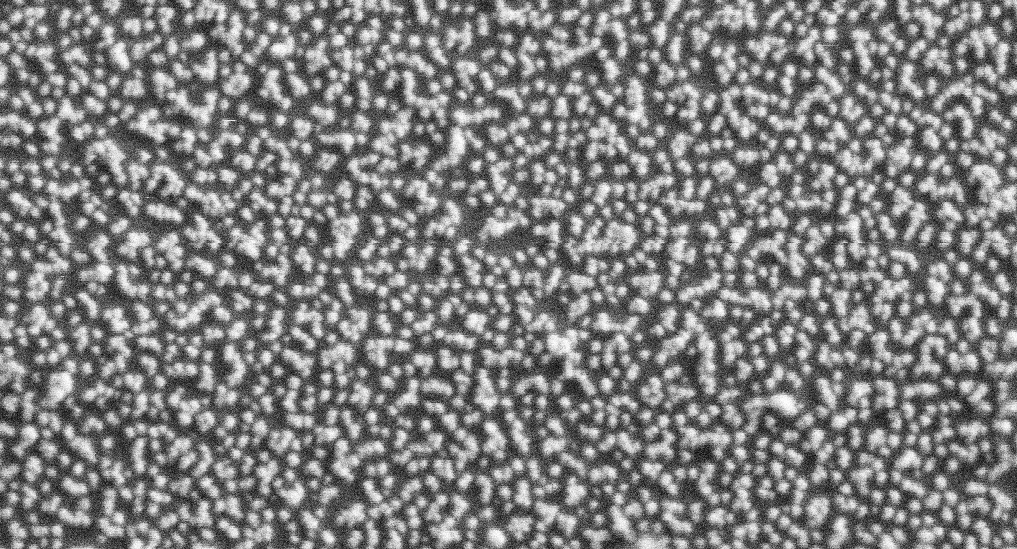
\includegraphics[width=10.5cm, height=7cm, keepaspectratio]{100000/f1_b1_100k11_high/f1_b1_100k11_high_cropped.png} }\\
\subfigure{\includegraphics[width=6.5cm]{100000/f1_b1_100k11_high/D_distribution} }
\subfigure{
\includegraphics[width=6.5cm, height=4.875cm, keepaspectratio, frame]{100000/f1_b1_100k11_high/f1_b1_100k11_high_adjusted.png} }
\subfigure{\includegraphics[width=6.5cm]{100000/f1_b1_100k11_high/D_scaled} }
\subfigure{\includegraphics[width=6.5cm]{100000/f1_b1_100k11_high/Brightness_distribution.png} }
\label{semimg0}
\caption*{\hyperlink{covtableaug_13_12}{\color{blue} \small \ttfamily f1\_b1\_100k11\_high}: SEM image, raw (top)/size-corrected (bottom), diam histograms, binary, grayscale.\\Cropped: {\bf True} \;\; BW coverage: {\bf 35.62} \:\: corr coverage: {\bf 46.29} \:\: hex fillfrac: {\bf 35.86} \:\: man-adjustment: {\bf \color{blue}{Yes}}}
\end{figure}
\newpage

\begin{textblock}{5}(4,1.0)
{\bf \textsc{aug\_13\_12}}
\hspace{4.5cm}
\hyperlink{covtableaug_13_12}{\color{blue} \large \ttfamily f1\_b1\_100k11\_low}
\end{textblock}

\begin{figure}[h!]\centering
\hypertarget{histf1_b1_100k11_low}{\;}
\subfigure{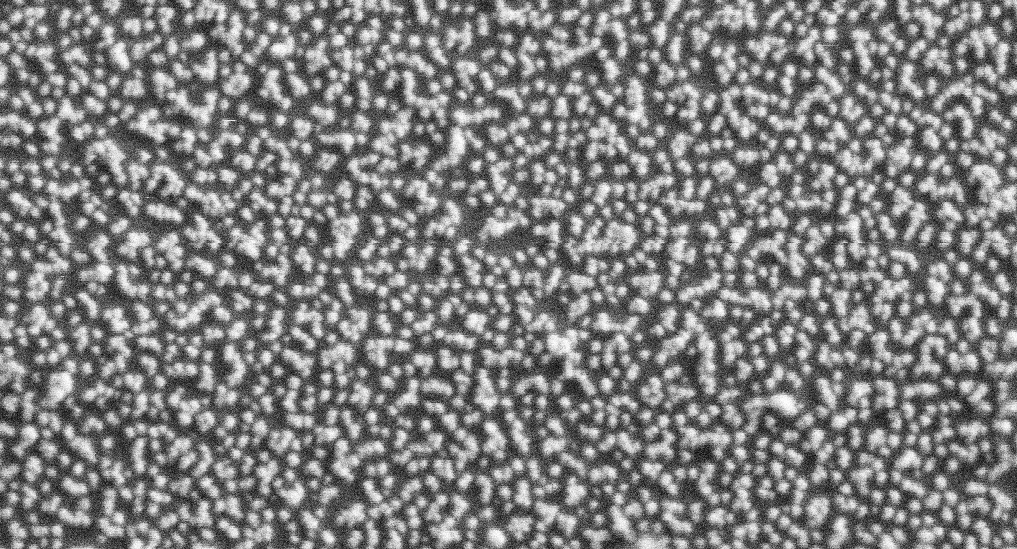
\includegraphics[width=10.5cm, height=7cm, keepaspectratio]{100000/f1_b1_100k11_low/f1_b1_100k11_low_cropped.png} }\\
\subfigure{\includegraphics[width=6.5cm]{100000/f1_b1_100k11_low/D_distribution} }
\subfigure{
\includegraphics[width=6.5cm, height=4.875cm, keepaspectratio, frame]{100000/f1_b1_100k11_low/f1_b1_100k11_low_adjusted.png} }
\subfigure{\includegraphics[width=6.5cm]{100000/f1_b1_100k11_low/D_scaled} }
\subfigure{\includegraphics[width=6.5cm]{100000/f1_b1_100k11_low/Brightness_distribution.png} }
\label{semimg1}
\caption*{\hyperlink{covtableaug_13_12}{\color{blue} \small \ttfamily f1\_b1\_100k11\_low}: SEM image, raw (top)/size-corrected (bottom), diam histograms, binary, grayscale.\\Cropped: {\bf True} \;\; BW coverage: {\bf 38.27} \:\: corr coverage: {\bf 46.15} \:\: hex fillfrac: {\bf 38.06} \:\: man-adjustment: {\bf \color{blue}{Yes}}}
\end{figure}
\newpage

\begin{textblock}{5}(4,1.0)
{\bf \textsc{aug\_13\_12}}
\hspace{4.5cm}
\hyperlink{covtableaug_13_12}{\color{blue} \large \ttfamily f1\_b1\_15k21\_high}
\end{textblock}

\begin{figure}[h!]\centering
\hypertarget{histf1_b1_15k21_high}{\;}
\subfigure{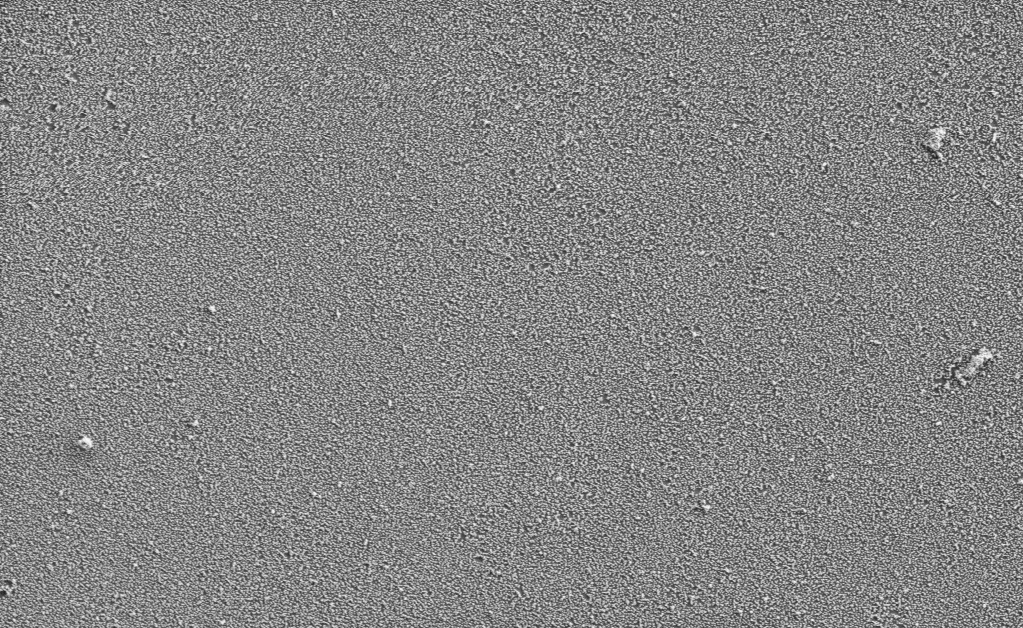
\includegraphics[width=10.5cm, height=7cm, keepaspectratio]{15000/f1_b1_15k21_high/f1_b1_15k21_high_cropped.png} }\\
\subfigure{\includegraphics[width=6.5cm]{15000/f1_b1_15k21_high/D_distribution} }
\subfigure{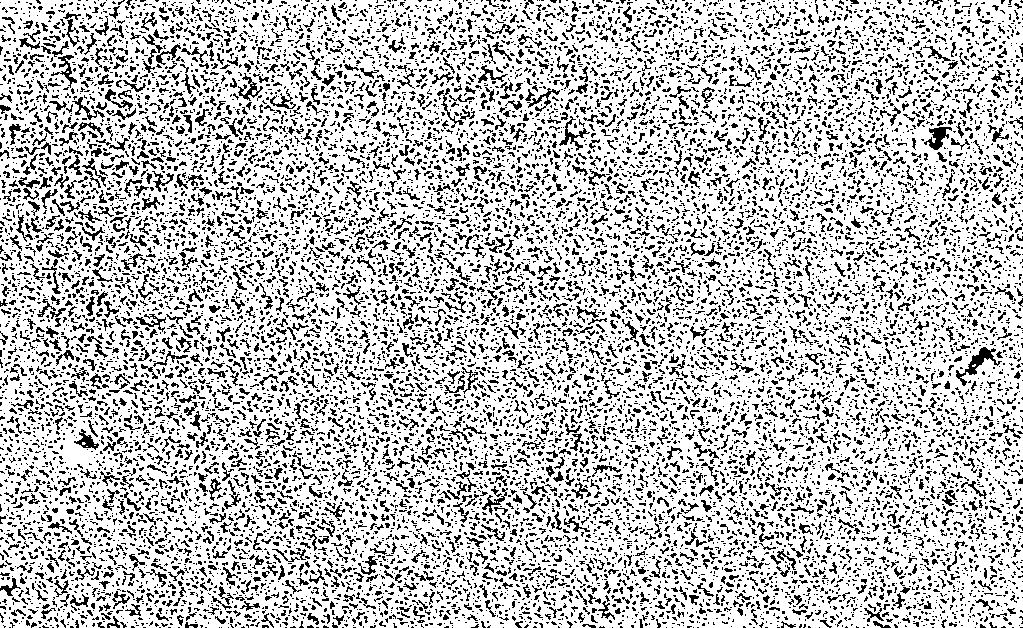
\includegraphics[width=6.5cm, height=4.875cm, keepaspectratio, frame]{15000/f1_b1_15k21_high/f1_b1_15k21_high_adjusted.png} }
\subfigure{\includegraphics[width=6.5cm]{15000/f1_b1_15k21_high/D_scaled} }
\subfigure{\includegraphics[width=6.5cm]{15000/f1_b1_15k21_high/Brightness_distribution.png} }
\label{semimg2}
\caption*{\hyperlink{covtableaug_13_12}{\color{blue} \small \ttfamily f1\_b1\_15k21\_high}: SEM image, raw (top)/size-corrected (bottom), diam histograms, binary, grayscale.\\Cropped: {\bf True} \;\; BW coverage: {\bf 24.28} \:\: corr coverage: {\bf 84.39} \:\: hex fillfrac: {\bf 17.91} \:\: man-adjustment: {\bf \color{blue}{Yes}}}
\end{figure}
\newpage

\begin{textblock}{5}(4,1.0)
{\bf \textsc{aug\_13\_12}}
\hspace{4.5cm}
\hyperlink{covtableaug_13_12}{\color{blue} \large \ttfamily f1\_b1\_15k21\_low}
\end{textblock}

\begin{figure}[h!]\centering
\hypertarget{histf1_b1_15k21_low}{\;}
\subfigure{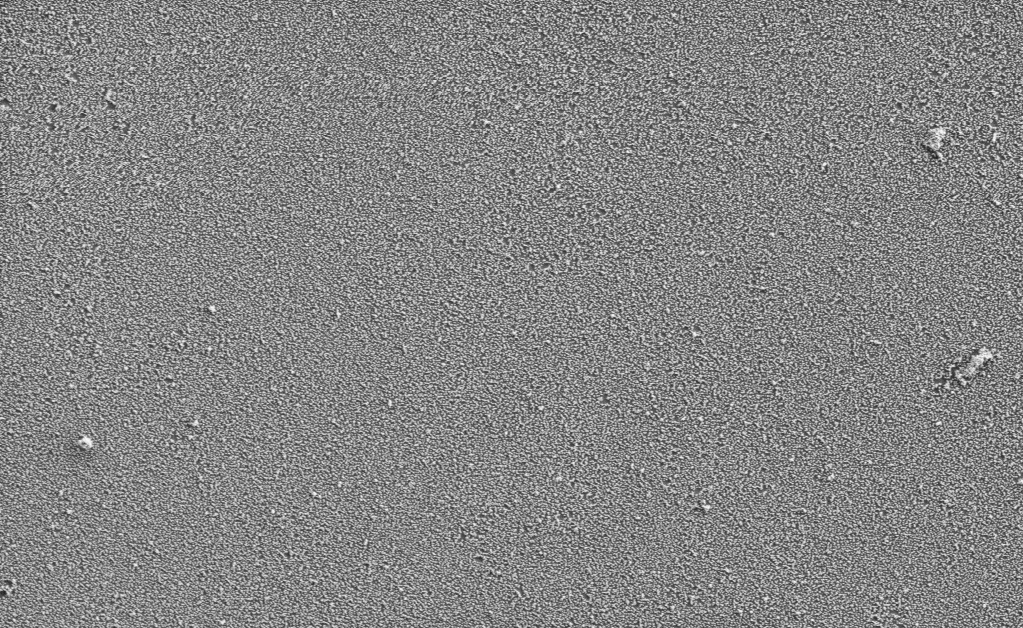
\includegraphics[width=10.5cm, height=7cm, keepaspectratio]{15000/f1_b1_15k21_low/f1_b1_15k21_low_cropped.png} }\\
\subfigure{\includegraphics[width=6.5cm]{15000/f1_b1_15k21_low/D_distribution} }
\subfigure{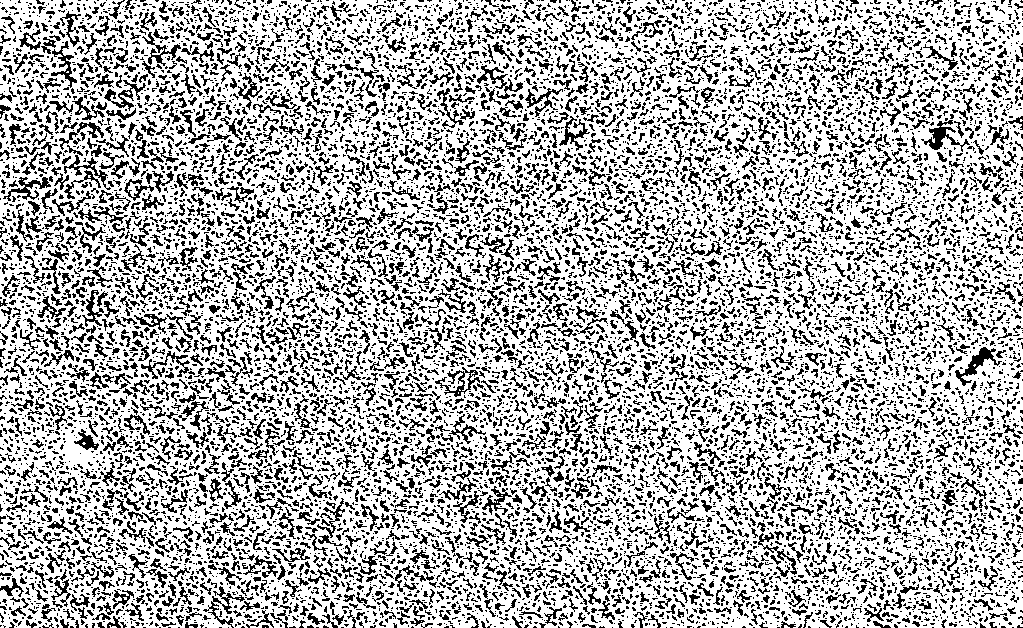
\includegraphics[width=6.5cm, height=4.875cm, keepaspectratio, frame]{15000/f1_b1_15k21_low/f1_b1_15k21_low_adjusted.png} }
\subfigure{\includegraphics[width=6.5cm]{15000/f1_b1_15k21_low/D_scaled} }
\subfigure{\includegraphics[width=6.5cm]{15000/f1_b1_15k21_low/Brightness_distribution.png} }
\label{semimg3}
\caption*{\hyperlink{covtableaug_13_12}{\color{blue} \small \ttfamily f1\_b1\_15k21\_low}: SEM image, raw (top)/size-corrected (bottom), diam histograms, binary, grayscale.\\Cropped: {\bf True} \;\; BW coverage: {\bf 29.57} \:\: corr coverage: {\bf 102.78} \:\: hex fillfrac: {\bf 16.76} \:\: man-adjustment: {\bf \color{blue}{Yes}}}
\end{figure}
\newpage

\begin{textblock}{5}(4,1.0)
{\bf \textsc{aug\_13\_12}}
\hspace{4.5cm}
\hyperlink{covtableaug_13_12}{\color{blue} \large \ttfamily f1\_b1\_30k1kx1\_high}
\end{textblock}

\begin{figure}[h!]\centering
\hypertarget{histf1_b1_30k1kx1_high}{\;}
\subfigure{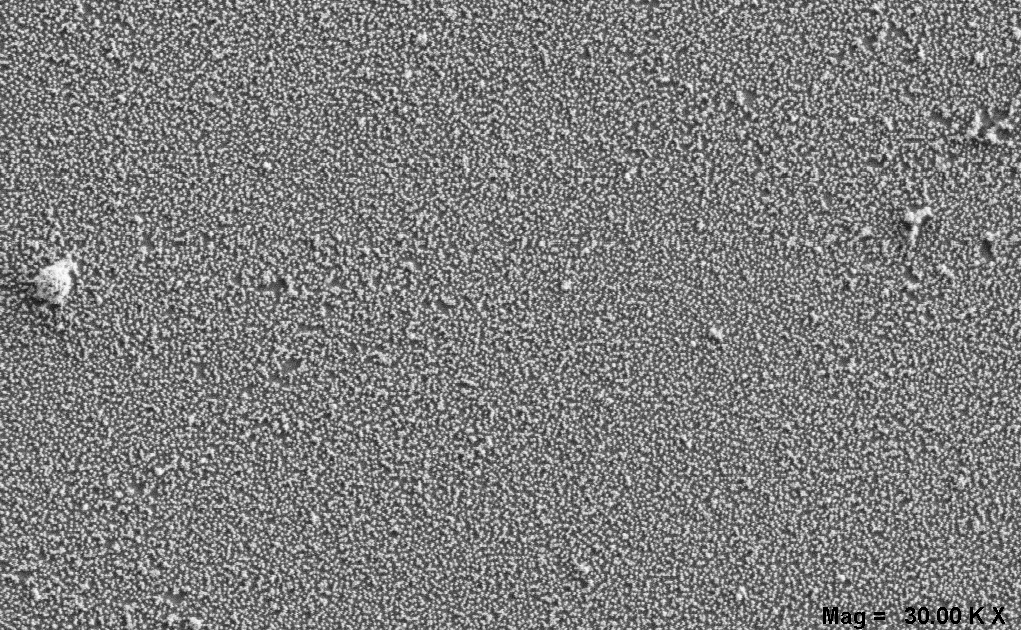
\includegraphics[width=10.5cm, height=7cm, keepaspectratio]{30000/f1_b1_30k1kx1_high/f1_b1_30k1kx1_high_cropped.png} }\\
\subfigure{\includegraphics[width=6.5cm]{30000/f1_b1_30k1kx1_high/D_distribution} }
\subfigure{
\includegraphics[width=6.5cm, height=4.875cm, keepaspectratio, frame]{30000/f1_b1_30k1kx1_high/f1_b1_30k1kx1_high_adjusted.png} }
\subfigure{\includegraphics[width=6.5cm]{30000/f1_b1_30k1kx1_high/D_scaled} }
\subfigure{\includegraphics[width=6.5cm]{30000/f1_b1_30k1kx1_high/Brightness_distribution.png} }
\label{semimg4}
\caption*{\hyperlink{covtableaug_13_12}{\color{blue} \small \ttfamily f1\_b1\_30k1kx1\_high}: SEM image, raw (top)/size-corrected (bottom), diam histograms, binary, grayscale.\\Cropped: {\bf True} \;\; BW coverage: {\bf 43.56} \:\: corr coverage: {\bf 220.69} \:\: hex fillfrac: {\bf 10.87} \:\: man-adjustment: {\bf \color{blue}{Yes}}}
\end{figure}
\newpage

\begin{textblock}{5}(4,1.0)
{\bf \textsc{aug\_13\_12}}
\hspace{4.5cm}
\hyperlink{covtableaug_13_12}{\color{blue} \large \ttfamily f1\_b1\_30k1kx1\_low}
\end{textblock}

\begin{figure}[h!]\centering
\hypertarget{histf1_b1_30k1kx1_low}{\;}
\subfigure{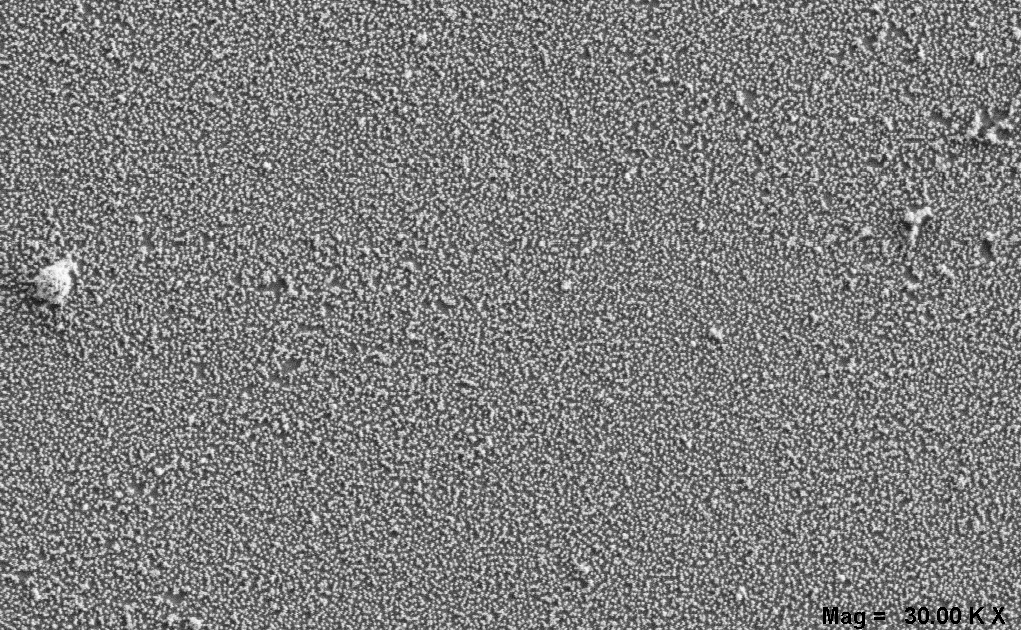
\includegraphics[width=10.5cm, height=7cm, keepaspectratio]{30000/f1_b1_30k1kx1_low/f1_b1_30k1kx1_low_cropped.png} }\\
\subfigure{\includegraphics[width=6.5cm]{30000/f1_b1_30k1kx1_low/D_distribution} }
\subfigure{
\includegraphics[width=6.5cm, height=4.875cm, keepaspectratio, frame]{30000/f1_b1_30k1kx1_low/f1_b1_30k1kx1_low_adjusted.png} }
\subfigure{\includegraphics[width=6.5cm]{30000/f1_b1_30k1kx1_low/D_scaled} }
\subfigure{\includegraphics[width=6.5cm]{30000/f1_b1_30k1kx1_low/Brightness_distribution.png} }
\label{semimg5}
\caption*{\hyperlink{covtableaug_13_12}{\color{blue} \small \ttfamily f1\_b1\_30k1kx1\_low}: SEM image, raw (top)/size-corrected (bottom), diam histograms, binary, grayscale.\\Cropped: {\bf True} \;\; BW coverage: {\bf 34.42} \:\: corr coverage: {\bf 174.38} \:\: hex fillfrac: {\bf 18.34} \:\: man-adjustment: {\bf \color{blue}{Yes}}}
\end{figure}
\newpage

\begin{textblock}{5}(4,1.0)
{\bf \textsc{aug\_13\_12}}
\hspace{4.5cm}
\hyperlink{covtableaug_13_12}{\color{blue} \large \ttfamily f1\_b1\_30k2kx1\_high}
\end{textblock}

\begin{figure}[h!]\centering
\hypertarget{histf1_b1_30k2kx1_high}{\;}
\subfigure{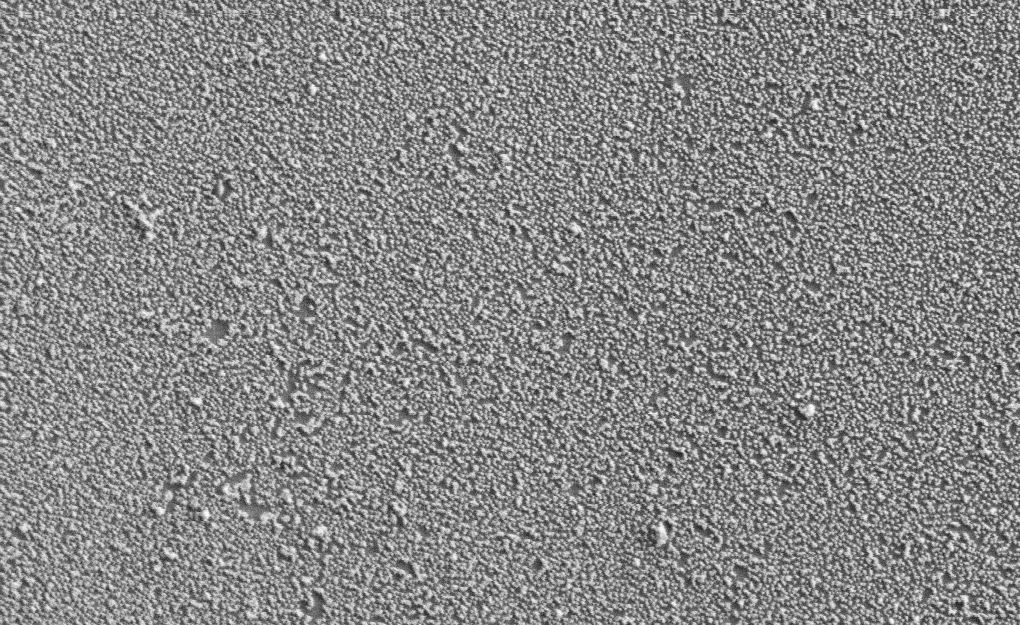
\includegraphics[width=10.5cm, height=7cm, keepaspectratio]{30000/f1_b1_30k2kx1_high/f1_b1_30k2kx1_high_cropped.png} }\\
\subfigure{\includegraphics[width=6.5cm]{30000/f1_b1_30k2kx1_high/D_distribution} }
\subfigure{
\includegraphics[width=6.5cm, height=4.875cm, keepaspectratio, frame]{30000/f1_b1_30k2kx1_high/f1_b1_30k2kx1_high_adjusted.png} }
\subfigure{\includegraphics[width=6.5cm]{30000/f1_b1_30k2kx1_high/D_scaled} }
\subfigure{\includegraphics[width=6.5cm]{30000/f1_b1_30k2kx1_high/Brightness_distribution.png} }
\label{semimg6}
\caption*{\hyperlink{covtableaug_13_12}{\color{blue} \small \ttfamily f1\_b1\_30k2kx1\_high}: SEM image, raw (top)/size-corrected (bottom), diam histograms, binary, grayscale.\\Cropped: {\bf True} \;\; BW coverage: {\bf 27.13} \:\: corr coverage: {\bf 137.48} \:\: hex fillfrac: {\bf 18.06} \:\: man-adjustment: {\bf \color{blue}{Yes}}}
\end{figure}
\newpage

\begin{textblock}{5}(4,1.0)
{\bf \textsc{aug\_13\_12}}
\hspace{4.5cm}
\hyperlink{covtableaug_13_12}{\color{blue} \large \ttfamily f1\_b1\_30k2kx1\_low}
\end{textblock}

\begin{figure}[h!]\centering
\hypertarget{histf1_b1_30k2kx1_low}{\;}
\subfigure{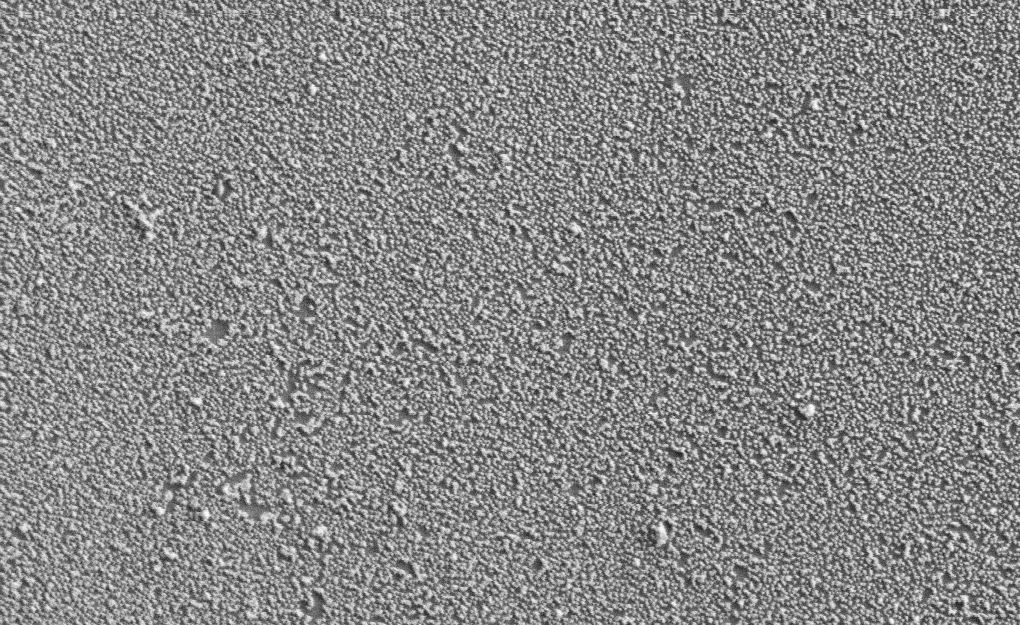
\includegraphics[width=10.5cm, height=7cm, keepaspectratio]{30000/f1_b1_30k2kx1_low/f1_b1_30k2kx1_low_cropped.png} }\\
\subfigure{\includegraphics[width=6.5cm]{30000/f1_b1_30k2kx1_low/D_distribution} }
\subfigure{
\includegraphics[width=6.5cm, height=4.875cm, keepaspectratio, frame]{30000/f1_b1_30k2kx1_low/f1_b1_30k2kx1_low_adjusted.png} }
\subfigure{\includegraphics[width=6.5cm]{30000/f1_b1_30k2kx1_low/D_scaled} }
\subfigure{\includegraphics[width=6.5cm]{30000/f1_b1_30k2kx1_low/Brightness_distribution.png} }
\label{semimg7}
\caption*{\hyperlink{covtableaug_13_12}{\color{blue} \small \ttfamily f1\_b1\_30k2kx1\_low}: SEM image, raw (top)/size-corrected (bottom), diam histograms, binary, grayscale.\\Cropped: {\bf True} \;\; BW coverage: {\bf 32.69} \:\: corr coverage: {\bf 165.64} \:\: hex fillfrac: {\bf 16.8} \:\: man-adjustment: {\bf \color{blue}{Yes}}}
\end{figure}
\newpage

\begin{textblock}{5}(4,1.0)
{\bf \textsc{aug\_13\_12}}
\hspace{4.5cm}
\hyperlink{covtableaug_13_12}{\color{blue} \large \ttfamily f1\_b1\_50kx31\_high}
\end{textblock}

\begin{figure}[h!]\centering
\hypertarget{histf1_b1_50kx31_high}{\;}
\subfigure{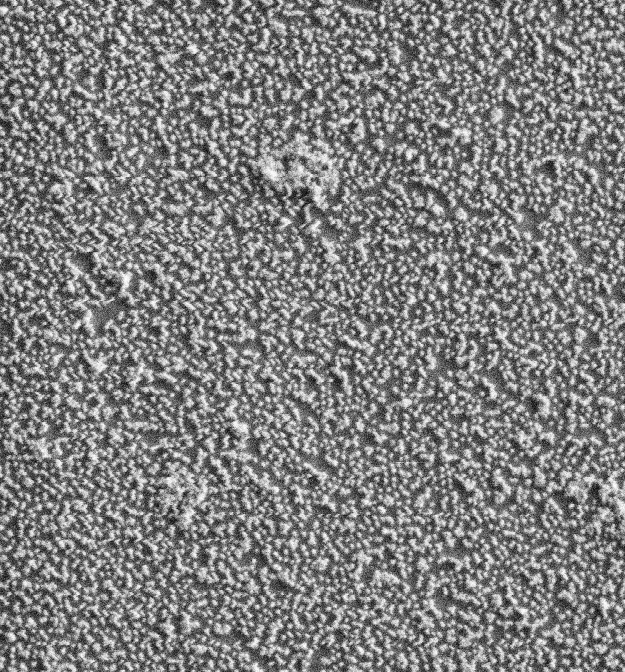
\includegraphics[width=10.5cm, height=7cm, keepaspectratio]{50000/f1_b1_50kx31_high/f1_b1_50kx31_high_cropped.png} }\\
\subfigure{\includegraphics[width=6.5cm]{50000/f1_b1_50kx31_high/D_distribution} }
\subfigure{
\includegraphics[width=6.5cm, height=4.875cm, keepaspectratio, frame]{50000/f1_b1_50kx31_high/f1_b1_50kx31_high_adjusted.png} }
\subfigure{\includegraphics[width=6.5cm]{50000/f1_b1_50kx31_high/D_scaled} }
\subfigure{\includegraphics[width=6.5cm]{50000/f1_b1_50kx31_high/Brightness_distribution.png} }
\label{semimg8}
\caption*{\hyperlink{covtableaug_13_12}{\color{blue} \small \ttfamily f1\_b1\_50kx31\_high}: SEM image, raw (top)/size-corrected (bottom), diam histograms, binary, grayscale.\\Cropped: {\bf True} \;\; BW coverage: {\bf 40.28} \:\: corr coverage: {\bf 70.01} \:\: hex fillfrac: {\bf 32.78} \:\: man-adjustment: {\bf \color{blue}{Yes}}}
\end{figure}
\newpage

\begin{textblock}{5}(4,1.0)
{\bf \textsc{aug\_13\_12}}
\hspace{4.5cm}
\hyperlink{covtableaug_13_12}{\color{blue} \large \ttfamily f1\_b1\_50kx31\_low}
\end{textblock}

\begin{figure}[h!]\centering
\hypertarget{histf1_b1_50kx31_low}{\;}
\subfigure{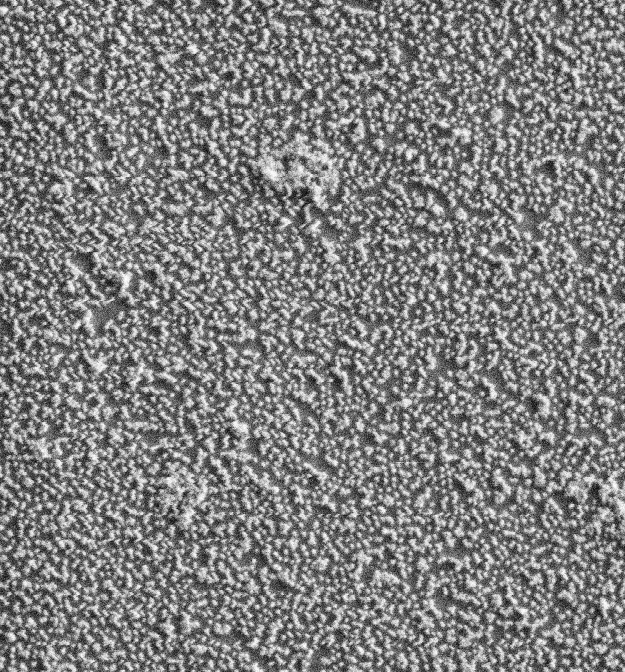
\includegraphics[width=10.5cm, height=7cm, keepaspectratio]{50000/f1_b1_50kx31_low/f1_b1_50kx31_low_cropped.png} }\\
\subfigure{\includegraphics[width=6.5cm]{50000/f1_b1_50kx31_low/D_distribution} }
\subfigure{
\includegraphics[width=6.5cm, height=4.875cm, keepaspectratio, frame]{50000/f1_b1_50kx31_low/f1_b1_50kx31_low_adjusted.png} }
\subfigure{\includegraphics[width=6.5cm]{50000/f1_b1_50kx31_low/D_scaled} }
\subfigure{\includegraphics[width=6.5cm]{50000/f1_b1_50kx31_low/Brightness_distribution.png} }
\label{semimg9}
\caption*{\hyperlink{covtableaug_13_12}{\color{blue} \small \ttfamily f1\_b1\_50kx31\_low}: SEM image, raw (top)/size-corrected (bottom), diam histograms, binary, grayscale.\\Cropped: {\bf True} \;\; BW coverage: {\bf 49.15} \:\: corr coverage: {\bf 56.85} \:\: hex fillfrac: {\bf 20.33} \:\: man-adjustment: {\bf \color{blue}{Yes}}}
\end{figure}
\newpage

\begin{textblock}{5}(4,1.0)
{\bf \textsc{aug\_13\_12}}
\hspace{4.5cm}
\hyperlink{covtableaug_13_12}{\color{blue} \large \ttfamily f1\_b2\_100k11\_high}
\end{textblock}

\begin{figure}[h!]\centering
\hypertarget{histf1_b2_100k11_high}{\;}
\subfigure{\includegraphics[width=10.5cm, height=7cm, keepaspectratio]{100000/f1_b2_100k11_high/f1_b2_100k11_high_cropped.png} }\\
\subfigure{\includegraphics[width=6.5cm]{100000/f1_b2_100k11_high/D_distribution} }
\subfigure{\includegraphics[width=6.5cm, height=4.875cm, keepaspectratio, frame]{100000/f1_b2_100k11_high/f1_b2_100k11_high_adjusted.png} }
\subfigure{\includegraphics[width=6.5cm]{100000/f1_b2_100k11_high/D_scaled} }
\subfigure{\includegraphics[width=6.5cm]{100000/f1_b2_100k11_high/Brightness_distribution.png} }
\label{semimg10}
\caption*{\hyperlink{covtableaug_13_12}{\color{blue} \small \ttfamily f1\_b2\_100k11\_high}: SEM image, raw (top)/size-corrected (bottom), diam histograms, binary, grayscale.\\Cropped: {\bf True} \;\; BW coverage: {\bf 26.94} \:\: corr coverage: {\bf 43.82} \:\: hex fillfrac: {\bf 30.27} \:\: man-adjustment: {\bf \color{blue}{Yes}}}
\end{figure}
\newpage

\begin{textblock}{5}(4,1.0)
{\bf \textsc{aug\_13\_12}}
\hspace{4.5cm}
\hyperlink{covtableaug_13_12}{\color{blue} \large \ttfamily f1\_b2\_100k11\_low}
\end{textblock}

\begin{figure}[h!]\centering
\hypertarget{histf1_b2_100k11_low}{\;}
\subfigure{\includegraphics[width=10.5cm, height=7cm, keepaspectratio]{100000/f1_b2_100k11_low/f1_b2_100k11_low_cropped.png} }\\
\subfigure{\includegraphics[width=6.5cm]{100000/f1_b2_100k11_low/D_distribution} }
\subfigure{\includegraphics[width=6.5cm, height=4.875cm, keepaspectratio, frame]{100000/f1_b2_100k11_low/f1_b2_100k11_low_adjusted.png} }
\subfigure{\includegraphics[width=6.5cm]{100000/f1_b2_100k11_low/D_scaled} }
\subfigure{\includegraphics[width=6.5cm]{100000/f1_b2_100k11_low/Brightness_distribution.png} }
\label{semimg11}
\caption*{\hyperlink{covtableaug_13_12}{\color{blue} \small \ttfamily f1\_b2\_100k11\_low}: SEM image, raw (top)/size-corrected (bottom), diam histograms, binary, grayscale.\\Cropped: {\bf True} \;\; BW coverage: {\bf 39.31} \:\: corr coverage: {\bf 46.75} \:\: hex fillfrac: {\bf 42.83} \:\: man-adjustment: {\bf \color{blue}{Yes}}}
\end{figure}
\newpage

\begin{textblock}{5}(4,1.0)
{\bf \textsc{aug\_13\_12}}
\hspace{4.5cm}
\hyperlink{covtableaug_13_12}{\color{blue} \large \ttfamily f1\_b2\_15k11\_high}
\end{textblock}

\begin{figure}[h!]\centering
\hypertarget{histf1_b2_15k11_high}{\;}
\subfigure{\includegraphics[width=10.5cm, height=7cm, keepaspectratio]{15000/f1_b2_15k11_high/f1_b2_15k11_high_cropped.png} }\\
\subfigure{\includegraphics[width=6.5cm]{15000/f1_b2_15k11_high/D_distribution} }
\subfigure{\includegraphics[width=6.5cm, height=4.875cm, keepaspectratio, frame]{15000/f1_b2_15k11_high/f1_b2_15k11_high_adjusted.png} }
\subfigure{\includegraphics[width=6.5cm]{15000/f1_b2_15k11_high/D_scaled} }
\subfigure{\includegraphics[width=6.5cm]{15000/f1_b2_15k11_high/Brightness_distribution.png} }
\label{semimg12}
\caption*{\hyperlink{covtableaug_13_12}{\color{blue} \small \ttfamily f1\_b2\_15k11\_high}: SEM image, raw (top)/size-corrected (bottom), diam histograms, binary, grayscale.\\Cropped: {\bf True} \;\; BW coverage: {\bf 14.05} \:\: corr coverage: {\bf 48.82} \:\: hex fillfrac: {\bf 13.89} \:\: man-adjustment: {\bf \color{blue}{Yes}}}
\end{figure}
\newpage

\begin{textblock}{5}(4,1.0)
{\bf \textsc{aug\_13\_12}}
\hspace{4.5cm}
\hyperlink{covtableaug_13_12}{\color{blue} \large \ttfamily f1\_b2\_15k11\_low}
\end{textblock}

\begin{figure}[h!]\centering
\hypertarget{histf1_b2_15k11_low}{\;}
\subfigure{\includegraphics[width=10.5cm, height=7cm, keepaspectratio]{15000/f1_b2_15k11_low/f1_b2_15k11_low_cropped.png} }\\
\subfigure{\includegraphics[width=6.5cm]{15000/f1_b2_15k11_low/D_distribution} }
\subfigure{\includegraphics[width=6.5cm, height=4.875cm, keepaspectratio, frame]{15000/f1_b2_15k11_low/f1_b2_15k11_low_adjusted.png} }
\subfigure{\includegraphics[width=6.5cm]{15000/f1_b2_15k11_low/D_scaled} }
\subfigure{\includegraphics[width=6.5cm]{15000/f1_b2_15k11_low/Brightness_distribution.png} }
\label{semimg13}
\caption*{\hyperlink{covtableaug_13_12}{\color{blue} \small \ttfamily f1\_b2\_15k11\_low}: SEM image, raw (top)/size-corrected (bottom), diam histograms, binary, grayscale.\\Cropped: {\bf True} \;\; BW coverage: {\bf 78.1} \:\: corr coverage: {\bf 269.49} \:\: hex fillfrac: {\bf 0.11} \:\: man-adjustment: {\bf \color{blue}{Yes}}}
\end{figure}
\newpage

\begin{textblock}{5}(4,1.0)
{\bf \textsc{aug\_13\_12}}
\hspace{4.5cm}
\hyperlink{covtableaug_13_12}{\color{blue} \large \ttfamily f1\_b2\_30k21\_high}
\end{textblock}

\begin{figure}[h!]\centering
\hypertarget{histf1_b2_30k21_high}{\;}
\subfigure{\includegraphics[width=10.5cm, height=7cm, keepaspectratio]{30000/f1_b2_30k21_high/f1_b2_30k21_high_cropped.png} }\\
\subfigure{\includegraphics[width=6.5cm]{30000/f1_b2_30k21_high/D_distribution} }
\subfigure{\includegraphics[width=6.5cm, height=4.875cm, keepaspectratio, frame]{30000/f1_b2_30k21_high/f1_b2_30k21_high_adjusted.png} }
\subfigure{\includegraphics[width=6.5cm]{30000/f1_b2_30k21_high/D_scaled} }
\subfigure{\includegraphics[width=6.5cm]{30000/f1_b2_30k21_high/Brightness_distribution.png} }
\label{semimg14}
\caption*{\hyperlink{covtableaug_13_12}{\color{blue} \small \ttfamily f1\_b2\_30k21\_high}: SEM image, raw (top)/size-corrected (bottom), diam histograms, binary, grayscale.\\Cropped: {\bf True} \;\; BW coverage: {\bf 16.47} \:\: corr coverage: {\bf 83.98} \:\: hex fillfrac: {\bf 17.35} \:\: man-adjustment: {\bf \color{blue}{Yes}}}
\end{figure}
\newpage

\begin{textblock}{5}(4,1.0)
{\bf \textsc{aug\_13\_12}}
\hspace{4.5cm}
\hyperlink{covtableaug_13_12}{\color{blue} \large \ttfamily f1\_b2\_30k21\_low}
\end{textblock}

\begin{figure}[h!]\centering
\hypertarget{histf1_b2_30k21_low}{\;}
\subfigure{\includegraphics[width=10.5cm, height=7cm, keepaspectratio]{30000/f1_b2_30k21_low/f1_b2_30k21_low_cropped.png} }\\
\subfigure{\includegraphics[width=6.5cm]{30000/f1_b2_30k21_low/D_distribution} }
\subfigure{\includegraphics[width=6.5cm, height=4.875cm, keepaspectratio, frame]{30000/f1_b2_30k21_low/f1_b2_30k21_low_adjusted.png} }
\subfigure{\includegraphics[width=6.5cm]{30000/f1_b2_30k21_low/D_scaled} }
\subfigure{\includegraphics[width=6.5cm]{30000/f1_b2_30k21_low/Brightness_distribution.png} }
\label{semimg15}
\caption*{\hyperlink{covtableaug_13_12}{\color{blue} \small \ttfamily f1\_b2\_30k21\_low}: SEM image, raw (top)/size-corrected (bottom), diam histograms, binary, grayscale.\\Cropped: {\bf True} \;\; BW coverage: {\bf 22.48} \:\: corr coverage: {\bf 113.89} \:\: hex fillfrac: {\bf 22.81} \:\: man-adjustment: {\bf \color{blue}{Yes}}}
\end{figure}
\newpage

\begin{textblock}{5}(4,1.0)
{\bf \textsc{aug\_13\_12}}
\hspace{4.5cm}
\hyperlink{covtableaug_13_12}{\color{blue} \large \ttfamily f1\_b2\_50k11\_high}
\end{textblock}

\begin{figure}[h!]\centering
\hypertarget{histf1_b2_50k11_high}{\;}
\subfigure{\includegraphics[width=10.5cm, height=7cm, keepaspectratio]{50000/f1_b2_50k11_high/f1_b2_50k11_high_cropped.png} }\\
\subfigure{\includegraphics[width=6.5cm]{50000/f1_b2_50k11_high/D_distribution} }
\subfigure{\includegraphics[width=6.5cm, height=4.875cm, keepaspectratio, frame]{50000/f1_b2_50k11_high/f1_b2_50k11_high_adjusted.png} }
\subfigure{\includegraphics[width=6.5cm]{50000/f1_b2_50k11_high/D_scaled} }
\subfigure{\includegraphics[width=6.5cm]{50000/f1_b2_50k11_high/Brightness_distribution.png} }
\label{semimg16}
\caption*{\hyperlink{covtableaug_13_12}{\color{blue} \small \ttfamily f1\_b2\_50k11\_high}: SEM image, raw (top)/size-corrected (bottom), diam histograms, binary, grayscale.\\Cropped: {\bf True} \;\; BW coverage: {\bf 25.48} \:\: corr coverage: {\bf 48.23} \:\: hex fillfrac: {\bf 28.29} \:\: man-adjustment: {\bf \color{blue}{Yes}}}
\end{figure}
\newpage

\begin{textblock}{5}(4,1.0)
{\bf \textsc{aug\_13\_12}}
\hspace{4.5cm}
\hyperlink{covtableaug_13_12}{\color{blue} \large \ttfamily f1\_b2\_50k11\_low}
\end{textblock}

\begin{figure}[h!]\centering
\hypertarget{histf1_b2_50k11_low}{\;}
\subfigure{\includegraphics[width=10.5cm, height=7cm, keepaspectratio]{50000/f1_b2_50k11_low/f1_b2_50k11_low_cropped.png} }\\
\subfigure{\includegraphics[width=6.5cm]{50000/f1_b2_50k11_low/D_distribution} }
\subfigure{\includegraphics[width=6.5cm, height=4.875cm, keepaspectratio, frame]{50000/f1_b2_50k11_low/f1_b2_50k11_low_adjusted.png} }
\subfigure{\includegraphics[width=6.5cm]{50000/f1_b2_50k11_low/D_scaled} }
\subfigure{\includegraphics[width=6.5cm]{50000/f1_b2_50k11_low/Brightness_distribution.png} }
\label{semimg17}
\caption*{\hyperlink{covtableaug_13_12}{\color{blue} \small \ttfamily f1\_b2\_50k11\_low}: SEM image, raw (top)/size-corrected (bottom), diam histograms, binary, grayscale.\\Cropped: {\bf True} \;\; BW coverage: {\bf 35.65} \:\: corr coverage: {\bf 37.43} \:\: hex fillfrac: {\bf 38.11} \:\: man-adjustment: {\bf \color{blue}{Yes}}}
\end{figure}
\newpage

\begin{textblock}{5}(4,1.0)
{\bf \textsc{aug\_13\_12}}
\hspace{4.5cm}
\hyperlink{covtableaug_13_12}{\color{blue} \large \ttfamily f1\_b2\_5k21\_high}
\end{textblock}

\begin{figure}[h!]\centering
\hypertarget{histf1_b2_5k21_high}{\;}
\subfigure{\includegraphics[width=10.5cm, height=7cm, keepaspectratio]{5000/f1_b2_5k21_high/f1_b2_5k21_high_cropped.png} }\\
\subfigure{\includegraphics[width=6.5cm]{5000/f1_b2_5k21_high/D_distribution} }
\subfigure{\includegraphics[width=6.5cm, height=4.875cm, keepaspectratio, frame]{5000/f1_b2_5k21_high/f1_b2_5k21_high_adjusted.png} }
\subfigure{\includegraphics[width=6.5cm]{5000/f1_b2_5k21_high/D_scaled} }
\subfigure{\includegraphics[width=6.5cm]{5000/f1_b2_5k21_high/Brightness_distribution.png} }
\label{semimg18}
\caption*{\hyperlink{covtableaug_13_12}{\color{blue} \small \ttfamily f1\_b2\_5k21\_high}: SEM image, raw (top)/size-corrected (bottom), diam histograms, binary, grayscale.\\Cropped: {\bf True} \;\; BW coverage: {\bf 1.5} \:\: corr coverage: {\bf 0.66} \:\: hex fillfrac: {\bf 1.58} \:\: man-adjustment: {\bf \color{blue}{Yes}}}
\end{figure}
\newpage

\begin{textblock}{5}(4,1.0)
{\bf \textsc{aug\_13\_12}}
\hspace{4.5cm}
\hyperlink{covtableaug_13_12}{\color{blue} \large \ttfamily f2\_b1\_100k21\_high}
\end{textblock}

\begin{figure}[h!]\centering
\hypertarget{histf2_b1_100k21_high}{\;}
\subfigure{\includegraphics[width=10.5cm, height=7cm, keepaspectratio]{100000/f2_b1_100k21_high/f2_b1_100k21_high_cropped.png} }\\
\subfigure{\includegraphics[width=6.5cm]{100000/f2_b1_100k21_high/D_distribution} }
\subfigure{\includegraphics[width=6.5cm, height=4.875cm, keepaspectratio, frame]{100000/f2_b1_100k21_high/f2_b1_100k21_high_adjusted.png} }
\subfigure{\includegraphics[width=6.5cm]{100000/f2_b1_100k21_high/D_scaled} }
\subfigure{\includegraphics[width=6.5cm]{100000/f2_b1_100k21_high/Brightness_distribution.png} }
\label{semimg19}
\caption*{\hyperlink{covtableaug_13_12}{\color{blue} \small \ttfamily f2\_b1\_100k21\_high}: SEM image, raw (top)/size-corrected (bottom), diam histograms, binary, grayscale.\\Cropped: {\bf True} \;\; BW coverage: {\bf 17.65} \:\: corr coverage: {\bf 32.89} \:\: hex fillfrac: {\bf 19.86} \:\: man-adjustment: {\bf \color{blue}{Yes}}}
\end{figure}
\newpage

\begin{textblock}{5}(4,1.0)
{\bf \textsc{aug\_13\_12}}
\hspace{4.5cm}
\hyperlink{covtableaug_13_12}{\color{blue} \large \ttfamily f2\_b1\_100k21\_low}
\end{textblock}

\begin{figure}[h!]\centering
\hypertarget{histf2_b1_100k21_low}{\;}
\subfigure{\includegraphics[width=10.5cm, height=7cm, keepaspectratio]{100000/f2_b1_100k21_low/f2_b1_100k21_low_cropped.png} }\\
\subfigure{\includegraphics[width=6.5cm]{100000/f2_b1_100k21_low/D_distribution} }
\subfigure{\includegraphics[width=6.5cm, height=4.875cm, keepaspectratio, frame]{100000/f2_b1_100k21_low/f2_b1_100k21_low_adjusted.png} }
\subfigure{\includegraphics[width=6.5cm]{100000/f2_b1_100k21_low/D_scaled} }
\subfigure{\includegraphics[width=6.5cm]{100000/f2_b1_100k21_low/Brightness_distribution.png} }
\label{semimg20}
\caption*{\hyperlink{covtableaug_13_12}{\color{blue} \small \ttfamily f2\_b1\_100k21\_low}: SEM image, raw (top)/size-corrected (bottom), diam histograms, binary, grayscale.\\Cropped: {\bf True} \;\; BW coverage: {\bf 28.86} \:\: corr coverage: {\bf 32.68} \:\: hex fillfrac: {\bf 29.8} \:\: man-adjustment: {\bf \color{blue}{Yes}}}
\end{figure}
\newpage

\begin{textblock}{5}(4,1.0)
{\bf \textsc{aug\_13\_12}}
\hspace{4.5cm}
\hyperlink{covtableaug_13_12}{\color{blue} \large \ttfamily f2\_b1\_15k\_highres\_9scan\_11int1\_high}
\end{textblock}

\begin{figure}[h!]\centering
\hypertarget{histf2_b1_15k_highres_9scan_11int1_high}{\;}
\subfigure{\includegraphics[width=10.5cm, height=7cm, keepaspectratio]{15000/f2_b1_15k_highres_9scan_11int1_high/f2_b1_15k_highres_9scan_11int1_high_cropped.png} }\\
\subfigure{\includegraphics[width=6.5cm]{15000/f2_b1_15k_highres_9scan_11int1_high/D_distribution} }
\subfigure{\includegraphics[width=6.5cm, height=4.875cm, keepaspectratio, frame]{15000/f2_b1_15k_highres_9scan_11int1_high/f2_b1_15k_highres_9scan_11int1_high_adjusted.png} }
\subfigure{\includegraphics[width=6.5cm]{15000/f2_b1_15k_highres_9scan_11int1_high/D_scaled} }
\subfigure{\includegraphics[width=6.5cm]{15000/f2_b1_15k_highres_9scan_11int1_high/Brightness_distribution.png} }
\label{semimg21}
\caption*{\hyperlink{covtableaug_13_12}{\color{blue} \small \ttfamily f2\_b1\_15k\_highres\_9scan\_11int1\_high}: SEM image, raw (top)/size-corrected (bottom), diam histograms, binary, grayscale.\\Cropped: {\bf True} \;\; BW coverage: {\bf 11.34} \:\: corr coverage: {\bf 39.42} \:\: hex fillfrac: {\bf 11.73} \:\: man-adjustment: {\bf \color{blue}{Yes}}}
\end{figure}
\newpage

\begin{textblock}{5}(4,1.0)
{\bf \textsc{aug\_13\_12}}
\hspace{4.5cm}
\hyperlink{covtableaug_13_12}{\color{blue} \large \ttfamily f2\_b1\_15k\_highres\_9scan\_11int1\_low}
\end{textblock}

\begin{figure}[h!]\centering
\hypertarget{histf2_b1_15k_highres_9scan_11int1_low}{\;}
\subfigure{\includegraphics[width=10.5cm, height=7cm, keepaspectratio]{15000/f2_b1_15k_highres_9scan_11int1_low/f2_b1_15k_highres_9scan_11int1_low_cropped.png} }\\
\subfigure{\includegraphics[width=6.5cm]{15000/f2_b1_15k_highres_9scan_11int1_low/D_distribution} }
\subfigure{\includegraphics[width=6.5cm, height=4.875cm, keepaspectratio, frame]{15000/f2_b1_15k_highres_9scan_11int1_low/f2_b1_15k_highres_9scan_11int1_low_adjusted.png} }
\subfigure{\includegraphics[width=6.5cm]{15000/f2_b1_15k_highres_9scan_11int1_low/D_scaled} }
\subfigure{\includegraphics[width=6.5cm]{15000/f2_b1_15k_highres_9scan_11int1_low/Brightness_distribution.png} }
\label{semimg22}
\caption*{\hyperlink{covtableaug_13_12}{\color{blue} \small \ttfamily f2\_b1\_15k\_highres\_9scan\_11int1\_low}: SEM image, raw (top)/size-corrected (bottom), diam histograms, binary, grayscale.\\Cropped: {\bf True} \;\; BW coverage: {\bf 20.31} \:\: corr coverage: {\bf 70.57} \:\: hex fillfrac: {\bf 16.72} \:\: man-adjustment: {\bf \color{blue}{Yes}}}
\end{figure}
\newpage

\begin{textblock}{5}(4,1.0)
{\bf \textsc{aug\_13\_12}}
\hspace{4.5cm}
\hyperlink{covtableaug_13_12}{\color{blue} \large \ttfamily f2\_b1\_30k31\_high}
\end{textblock}

\begin{figure}[h!]\centering
\hypertarget{histf2_b1_30k31_high}{\;}
\subfigure{\includegraphics[width=10.5cm, height=7cm, keepaspectratio]{30000/f2_b1_30k31_high/f2_b1_30k31_high_cropped.png} }\\
\subfigure{\includegraphics[width=6.5cm]{30000/f2_b1_30k31_high/D_distribution} }
\subfigure{\includegraphics[width=6.5cm, height=4.875cm, keepaspectratio, frame]{30000/f2_b1_30k31_high/f2_b1_30k31_high_adjusted.png} }
\subfigure{\includegraphics[width=6.5cm]{30000/f2_b1_30k31_high/D_scaled} }
\subfigure{\includegraphics[width=6.5cm]{30000/f2_b1_30k31_high/Brightness_distribution.png} }
\label{semimg23}
\caption*{\hyperlink{covtableaug_13_12}{\color{blue} \small \ttfamily f2\_b1\_30k31\_high}: SEM image, raw (top)/size-corrected (bottom), diam histograms, binary, grayscale.\\Cropped: {\bf True} \;\; BW coverage: {\bf 15.64} \:\: corr coverage: {\bf 79.23} \:\: hex fillfrac: {\bf 16.3} \:\: man-adjustment: {\bf \color{blue}{Yes}}}
\end{figure}
\newpage

\begin{textblock}{5}(4,1.0)
{\bf \textsc{aug\_13\_12}}
\hspace{4.5cm}
\hyperlink{covtableaug_13_12}{\color{blue} \large \ttfamily f2\_b1\_30k31\_low}
\end{textblock}

\begin{figure}[h!]\centering
\hypertarget{histf2_b1_30k31_low}{\;}
\subfigure{\includegraphics[width=10.5cm, height=7cm, keepaspectratio]{30000/f2_b1_30k31_low/f2_b1_30k31_low_cropped.png} }\\
\subfigure{\includegraphics[width=6.5cm]{30000/f2_b1_30k31_low/D_distribution} }
\subfigure{\includegraphics[width=6.5cm, height=4.875cm, keepaspectratio, frame]{30000/f2_b1_30k31_low/f2_b1_30k31_low_adjusted.png} }
\subfigure{\includegraphics[width=6.5cm]{30000/f2_b1_30k31_low/D_scaled} }
\subfigure{\includegraphics[width=6.5cm]{30000/f2_b1_30k31_low/Brightness_distribution.png} }
\label{semimg24}
\caption*{\hyperlink{covtableaug_13_12}{\color{blue} \small \ttfamily f2\_b1\_30k31\_low}: SEM image, raw (top)/size-corrected (bottom), diam histograms, binary, grayscale.\\Cropped: {\bf True} \;\; BW coverage: {\bf 19.61} \:\: corr coverage: {\bf 99.37} \:\: hex fillfrac: {\bf 19.96} \:\: man-adjustment: {\bf \color{blue}{Yes}}}
\end{figure}
\newpage

\begin{textblock}{5}(4,1.0)
{\bf \textsc{aug\_13\_12}}
\hspace{4.5cm}
\hyperlink{covtableaug_13_12}{\color{blue} \large \ttfamily f2\_b1\_50k21\_high}
\end{textblock}

\begin{figure}[h!]\centering
\hypertarget{histf2_b1_50k21_high}{\;}
\subfigure{\includegraphics[width=10.5cm, height=7cm, keepaspectratio]{50000/f2_b1_50k21_high/f2_b1_50k21_high_cropped.png} }\\
\subfigure{\includegraphics[width=6.5cm]{50000/f2_b1_50k21_high/D_distribution} }
\subfigure{\includegraphics[width=6.5cm, height=4.875cm, keepaspectratio, frame]{50000/f2_b1_50k21_high/f2_b1_50k21_high_adjusted.png} }
\subfigure{\includegraphics[width=6.5cm]{50000/f2_b1_50k21_high/D_scaled} }
\subfigure{\includegraphics[width=6.5cm]{50000/f2_b1_50k21_high/Brightness_distribution.png} }
\label{semimg25}
\caption*{\hyperlink{covtableaug_13_12}{\color{blue} \small \ttfamily f2\_b1\_50k21\_high}: SEM image, raw (top)/size-corrected (bottom), diam histograms, binary, grayscale.\\Cropped: {\bf True} \;\; BW coverage: {\bf 62.59} \:\: corr coverage: {\bf 60.04} \:\: hex fillfrac: {\bf 16.65} \:\: man-adjustment: {\bf \color{blue}{Yes}}}
\end{figure}
\newpage

\begin{textblock}{5}(4,1.0)
{\bf \textsc{aug\_13\_12}}
\hspace{4.5cm}
\hyperlink{covtableaug_13_12}{\color{blue} \large \ttfamily f2\_b1\_50k21\_low}
\end{textblock}

\begin{figure}[h!]\centering
\hypertarget{histf2_b1_50k21_low}{\;}
\subfigure{\includegraphics[width=10.5cm, height=7cm, keepaspectratio]{50000/f2_b1_50k21_low/f2_b1_50k21_low_cropped.png} }\\
\subfigure{\includegraphics[width=6.5cm]{50000/f2_b1_50k21_low/D_distribution} }
\subfigure{\includegraphics[width=6.5cm, height=4.875cm, keepaspectratio, frame]{50000/f2_b1_50k21_low/f2_b1_50k21_low_adjusted.png} }
\subfigure{\includegraphics[width=6.5cm]{50000/f2_b1_50k21_low/D_scaled} }
\subfigure{\includegraphics[width=6.5cm]{50000/f2_b1_50k21_low/Brightness_distribution.png} }
\label{semimg26}
\caption*{\hyperlink{covtableaug_13_12}{\color{blue} \small \ttfamily f2\_b1\_50k21\_low}: SEM image, raw (top)/size-corrected (bottom), diam histograms, binary, grayscale.\\Cropped: {\bf True} \;\; BW coverage: {\bf 64.77} \:\: corr coverage: {\bf 61.65} \:\: hex fillfrac: {\bf 15.43} \:\: man-adjustment: {\bf \color{blue}{Yes}}}
\end{figure}
\newpage

\begin{textblock}{5}(4,1.0)
{\bf \textsc{aug\_13\_12}}
\hspace{4.5cm}
\hyperlink{covtableaug_13_12}{\color{blue} \large \ttfamily f2\_b2\_15k31\_high}
\end{textblock}

\begin{figure}[h!]\centering
\hypertarget{histf2_b2_15k31_high}{\;}
\subfigure{\includegraphics[width=10.5cm, height=7cm, keepaspectratio]{15000/f2_b2_15k31_high/f2_b2_15k31_high_cropped.png} }\\
\subfigure{\includegraphics[width=6.5cm]{15000/f2_b2_15k31_high/D_distribution} }
\subfigure{\includegraphics[width=6.5cm, height=4.875cm, keepaspectratio, frame]{15000/f2_b2_15k31_high/f2_b2_15k31_high_adjusted.png} }
\subfigure{\includegraphics[width=6.5cm]{15000/f2_b2_15k31_high/D_scaled} }
\subfigure{\includegraphics[width=6.5cm]{15000/f2_b2_15k31_high/Brightness_distribution.png} }
\label{semimg27}
\caption*{\hyperlink{covtableaug_13_12}{\color{blue} \small \ttfamily f2\_b2\_15k31\_high}: SEM image, raw (top)/size-corrected (bottom), diam histograms, binary, grayscale.\\Cropped: {\bf True} \;\; BW coverage: {\bf 7.38} \:\: corr coverage: {\bf 25.66} \:\: hex fillfrac: {\bf 7.28} \:\: man-adjustment: {\bf \color{blue}{Yes}}}
\end{figure}
\newpage

\begin{textblock}{5}(4,1.0)
{\bf \textsc{aug\_13\_12}}
\hspace{4.5cm}
\hyperlink{covtableaug_13_12}{\color{blue} \large \ttfamily f2\_b2\_15k31\_low}
\end{textblock}

\begin{figure}[h!]\centering
\hypertarget{histf2_b2_15k31_low}{\;}
\subfigure{\includegraphics[width=10.5cm, height=7cm, keepaspectratio]{15000/f2_b2_15k31_low/f2_b2_15k31_low_cropped.png} }\\
\subfigure{\includegraphics[width=6.5cm]{15000/f2_b2_15k31_low/D_distribution} }
\subfigure{\includegraphics[width=6.5cm, height=4.875cm, keepaspectratio, frame]{15000/f2_b2_15k31_low/f2_b2_15k31_low_adjusted.png} }
\subfigure{\includegraphics[width=6.5cm]{15000/f2_b2_15k31_low/D_scaled} }
\subfigure{\includegraphics[width=6.5cm]{15000/f2_b2_15k31_low/Brightness_distribution.png} }
\label{semimg28}
\caption*{\hyperlink{covtableaug_13_12}{\color{blue} \small \ttfamily f2\_b2\_15k31\_low}: SEM image, raw (top)/size-corrected (bottom), diam histograms, binary, grayscale.\\Cropped: {\bf True} \;\; BW coverage: {\bf 26.67} \:\: corr coverage: {\bf 92.68} \:\: hex fillfrac: {\bf 17.4} \:\: man-adjustment: {\bf \color{blue}{Yes}}}
\end{figure}
\newpage

\begin{textblock}{5}(4,1.0)
{\bf \textsc{aug\_13\_12}}
\hspace{4.5cm}
\hyperlink{covtableaug_13_12}{\color{blue} \large \ttfamily f2\_b2\_30k31\_high}
\end{textblock}

\begin{figure}[h!]\centering
\hypertarget{histf2_b2_30k31_high}{\;}
\subfigure{\includegraphics[width=10.5cm, height=7cm, keepaspectratio]{30000/f2_b2_30k31_high/f2_b2_30k31_high_cropped.png} }\\
\subfigure{\includegraphics[width=6.5cm]{30000/f2_b2_30k31_high/D_distribution} }
\subfigure{\includegraphics[width=6.5cm, height=4.875cm, keepaspectratio, frame]{30000/f2_b2_30k31_high/f2_b2_30k31_high_adjusted.png} }
\subfigure{\includegraphics[width=6.5cm]{30000/f2_b2_30k31_high/D_scaled} }
\subfigure{\includegraphics[width=6.5cm]{30000/f2_b2_30k31_high/Brightness_distribution.png} }
\label{semimg29}
\caption*{\hyperlink{covtableaug_13_12}{\color{blue} \small \ttfamily f2\_b2\_30k31\_high}: SEM image, raw (top)/size-corrected (bottom), diam histograms, binary, grayscale.\\Cropped: {\bf True} \;\; BW coverage: {\bf 5.03} \:\: corr coverage: {\bf 25.98} \:\: hex fillfrac: {\bf 4.78} \:\: man-adjustment: {\bf \color{blue}{Yes}}}
\end{figure}
\newpage

\begin{textblock}{5}(4,1.0)
{\bf \textsc{aug\_13\_12}}
\hspace{4.5cm}
\hyperlink{covtableaug_13_12}{\color{blue} \large \ttfamily f2\_b2\_30k31\_low}
\end{textblock}

\begin{figure}[h!]\centering
\hypertarget{histf2_b2_30k31_low}{\;}
\subfigure{\includegraphics[width=10.5cm, height=7cm, keepaspectratio]{30000/f2_b2_30k31_low/f2_b2_30k31_low_cropped.png} }\\
\subfigure{\includegraphics[width=6.5cm]{30000/f2_b2_30k31_low/D_distribution} }
\subfigure{\includegraphics[width=6.5cm, height=4.875cm, keepaspectratio, frame]{30000/f2_b2_30k31_low/f2_b2_30k31_low_adjusted.png} }
\subfigure{\includegraphics[width=6.5cm]{30000/f2_b2_30k31_low/D_scaled} }
\subfigure{\includegraphics[width=6.5cm]{30000/f2_b2_30k31_low/Brightness_distribution.png} }
\label{semimg30}
\caption*{\hyperlink{covtableaug_13_12}{\color{blue} \small \ttfamily f2\_b2\_30k31\_low}: SEM image, raw (top)/size-corrected (bottom), diam histograms, binary, grayscale.\\Cropped: {\bf True} \;\; BW coverage: {\bf 43.41} \:\: corr coverage: {\bf 219.96} \:\: hex fillfrac: {\bf 12.93} \:\: man-adjustment: {\bf \color{blue}{Yes}}}
\end{figure}
\newpage

\begin{textblock}{5}(4,1.0)
{\bf \textsc{aug\_13\_12}}
\hspace{4.5cm}
\hyperlink{covtableaug_13_12}{\color{blue} \large \ttfamily f2\_b2\_50k31\_high}
\end{textblock}

\begin{figure}[h!]\centering
\hypertarget{histf2_b2_50k31_high}{\;}
\subfigure{\includegraphics[width=10.5cm, height=7cm, keepaspectratio]{50000/f2_b2_50k31_high/f2_b2_50k31_high_cropped.png} }\\
\subfigure{\includegraphics[width=6.5cm]{50000/f2_b2_50k31_high/D_distribution} }
\subfigure{\includegraphics[width=6.5cm, height=4.875cm, keepaspectratio, frame]{50000/f2_b2_50k31_high/f2_b2_50k31_high_adjusted.png} }
\subfigure{\includegraphics[width=6.5cm]{50000/f2_b2_50k31_high/D_scaled} }
\subfigure{\includegraphics[width=6.5cm]{50000/f2_b2_50k31_high/Brightness_distribution.png} }
\label{semimg31}
\caption*{\hyperlink{covtableaug_13_12}{\color{blue} \small \ttfamily f2\_b2\_50k31\_high}: SEM image, raw (top)/size-corrected (bottom), diam histograms, binary, grayscale.\\Cropped: {\bf True} \;\; BW coverage: {\bf 16.14} \:\: corr coverage: {\bf 66.91} \:\: hex fillfrac: {\bf 19.3} \:\: man-adjustment: {\bf \color{blue}{Yes}}}
\end{figure}
\newpage

\begin{textblock}{5}(4,1.0)
{\bf \textsc{aug\_13\_12}}
\hspace{4.5cm}
\hyperlink{covtableaug_13_12}{\color{blue} \large \ttfamily f2\_b2\_50k31\_low}
\end{textblock}

\begin{figure}[h!]\centering
\hypertarget{histf2_b2_50k31_low}{\;}
\subfigure{\includegraphics[width=10.5cm, height=7cm, keepaspectratio]{50000/f2_b2_50k31_low/f2_b2_50k31_low_cropped.png} }\\
\subfigure{\includegraphics[width=6.5cm]{50000/f2_b2_50k31_low/D_distribution} }
\subfigure{\includegraphics[width=6.5cm, height=4.875cm, keepaspectratio, frame]{50000/f2_b2_50k31_low/f2_b2_50k31_low_adjusted.png} }
\subfigure{\includegraphics[width=6.5cm]{50000/f2_b2_50k31_low/D_scaled} }
\subfigure{\includegraphics[width=6.5cm]{50000/f2_b2_50k31_low/Brightness_distribution.png} }
\label{semimg32}
\caption*{\hyperlink{covtableaug_13_12}{\color{blue} \small \ttfamily f2\_b2\_50k31\_low}: SEM image, raw (top)/size-corrected (bottom), diam histograms, binary, grayscale.\\Cropped: {\bf True} \;\; BW coverage: {\bf 42.17} \:\: corr coverage: {\bf 41.2} \:\: hex fillfrac: {\bf 38.65} \:\: man-adjustment: {\bf \color{blue}{Yes}}}
\end{figure}
\newpage

\begin{textblock}{5}(4,1.0)
{\bf \textsc{aug\_13\_12}}
\hspace{4.5cm}
\hyperlink{covtableaug_13_12}{\color{blue} \large \ttfamily f2\_b2\_5k21\_high}
\end{textblock}

\begin{figure}[h!]\centering
\hypertarget{histf2_b2_5k21_high}{\;}
\subfigure{\includegraphics[width=10.5cm, height=7cm, keepaspectratio]{5000/f2_b2_5k21_high/f2_b2_5k21_high_cropped.png} }\\
\subfigure{\includegraphics[width=6.5cm]{5000/f2_b2_5k21_high/D_distribution} }
\subfigure{\includegraphics[width=6.5cm, height=4.875cm, keepaspectratio, frame]{5000/f2_b2_5k21_high/f2_b2_5k21_high_adjusted.png} }
\subfigure{\includegraphics[width=6.5cm]{5000/f2_b2_5k21_high/D_scaled} }
\subfigure{\includegraphics[width=6.5cm]{5000/f2_b2_5k21_high/Brightness_distribution.png} }
\label{semimg33}
\caption*{\hyperlink{covtableaug_13_12}{\color{blue} \small \ttfamily f2\_b2\_5k21\_high}: SEM image, raw (top)/size-corrected (bottom), diam histograms, binary, grayscale.\\Cropped: {\bf True} \;\; BW coverage: {\bf 1.25} \:\: corr coverage: {\bf 0.55} \:\: hex fillfrac: {\bf 1.31} \:\: man-adjustment: {\bf \color{blue}{Yes}}}
\end{figure}
\newpage



\end{document}